\newif\ifdblatexpdf \ifx\pdfoutput\undefined \else \ifx\pdfoutput\relax \else\ifnum\pdfoutput>0 \dblatexpdftrue \fi \fi \fi
% ------------------------------------------------------------
% Autogenerated LaTeX file for books
% db2latex RELEASE: 0.8pre1
% db2latex VERSION: $Id: VERSION.xml,v 1.6 2004/01/31 12:47:11 j-devenish Exp $
% fithesis VERSION: 1.40
% ------------------------------------------------------------
\def\clsclass{rapport3}
\documentclass{fithesis}
% --------------------------------------------
% MetaFont and MetaPost logo support
% --------------------------------------------
\usepackage{mflogo}
% --------------------------------------------
% Load fithesis param 
% --------------------------------------------
\thesistitle{Real-time Communication in Web Browser}
\thesissubtitle{Master thesis}
\thesisstudent{Pavel Smolka}
\thesiswoman{false}
\thesislang{en}
\thesisyear{2013}
\thesisfaculty{fi}
\thesisadvisor{doc.
      RNDr. Tom� Pitner, Ph.D.}
% --------------------------------------------
\label{idp8448}% --------------------------------------------
% Load graphicx package with pdf if needed 
% --------------------------------------------
\ifdblatexpdf
\usepackage[pdftex]{graphicx}
\pdfcompresslevel=9
\else
\usepackage{graphicx}
\fi
\usepackage{anysize}
\marginsize{3cm}{2.5cm}{3.5cm}{3.5cm}

\makeatletter
% redefine the listoffigures and listoftables so that the name of the chapter
% is printed whenever there are figures or tables from that chapter. encourage
% pagebreak prior to the name of the chapter (discourage orphans).
\let\save@@chapter\@chapter
\let\save@@l@figure\l@figure
\let\the@l@figure@leader\relax
\def\@chapter[#1]#2{\save@@chapter[{#1}]{#2}%
\addtocontents{lof}{\protect\def\the@l@figure@leader{\protect\pagebreak[0]\protect\contentsline{chapter}{\protect\numberline{\thechapter}#1}{}{\thepage}}}%
\addtocontents{lot}{\protect\def\the@l@figure@leader{\protect\pagebreak[0]\protect\contentsline{chapter}{\protect\numberline{\thechapter}#1}{}{\thepage}}}%
}
\renewcommand*\l@figure{\the@l@figure@leader\let\the@l@figure@leader\relax\save@@l@figure}
\let\l@table\l@figure
\makeatother
\usepackage{fancyhdr}
\renewcommand{\headrulewidth}{0.4pt}
\renewcommand{\footrulewidth}{0.4pt}
% Safeguard against long headers.
\IfFileExists{truncate.sty}{
\usepackage{truncate}
% Use an ellipsis when text would be larger than x% of the text width.
% Preserve left/right text alignment using \hfill (works for English).
\fancyhead[ol]{\truncate{0.49\textwidth}{\sl\leftmark}}
\fancyhead[er]{\truncate{0.49\textwidth}{\hfill\sl\rightmark}}
\fancyhead[el]{\truncate{0.49\textwidth}{\sl\leftmark}}
\fancyhead[or]{\truncate{0.49\textwidth}{\hfill\sl\rightmark}}
}{\typeout{WARNING: truncate.sty wasn't available and functionality was skipped.}}
\pagestyle{fancy}
% ---------------------- 
% Most Common Packages   
% ---------------------- 
\usepackage{latexsym}         
\usepackage{enumerate}         
\usepackage{fancybox}      
\usepackage{float}       
\usepackage{ragged2e}       
\usepackage{fancyvrb}         
\makeatletter\@namedef{FV@fontfamily@default}{\def\FV@FontScanPrep{}\def\FV@FontFamily{}}\makeatother
\fvset{obeytabs=true,tabsize=3}
\makeatletter
\let\dblatex@center\center\let\dblatex@endcenter\endcenter
\def\dblatex@nolistI{\leftmargin\leftmargini\topsep\z@ \parsep\parskip \itemsep\z@}
\def\center{\let\@listi\dblatex@nolistI\@listi\dblatex@center\let\@listi\@listI\@listi}
\def\endcenter{\dblatex@endcenter}
\makeatother
\usepackage{rotating}         
\usepackage{subfigure}         
\usepackage{tabularx}         
\usepackage{url}         
% --------------------------------------------
% Load hyperref package with pdf if needed 
% --------------------------------------------
\ifdblatexpdf
\usepackage[pdftex,bookmarksnumbered,colorlinks,backref,bookmarks,breaklinks,linktocpage,plainpages=false, pdfstartview=FitH, plainpages=false, pdfpagelabels, unicode]{hyperref}
\else
\usepackage[bookmarksnumbered,colorlinks,backref,bookmarks,breaklinks,linktocpage,plainpages=false, plainpages=false, pdfpagelabels]{hyperref}
\fi
% --------------------------------------------
% ----------------------------------------------
% Define a new LaTeX environment (adminipage)
% ----------------------------------------------
\newenvironment{admminipage}%
{ % this code corresponds to the \begin{adminipage} command
 \begin{Sbox}%
 \begin{minipage}%
} %done
{ % this code corresponds to the \end{adminipage} command
 \end{minipage}
 \end{Sbox}
 \fbox{\TheSbox}
} %done
% ----------------------------------------------
% Define a new LaTeX length (admlength)
% ----------------------------------------------
\newlength{\admlength}
% ----------------------------------------------
% Define a new LaTeX environment (admonition)
% With 2 parameters:
% #1 The file (e.g. note.pdf)
% #2 The caption
% ----------------------------------------------
\newenvironment{admonition}[2] 
{ % this code corresponds to the \begin{admonition} command
 \hspace{0mm}\newline\hspace*\fill\newline
 \noindent
 \setlength{\fboxsep}{5pt}
 \setlength{\admlength}{\linewidth}
 \addtolength{\admlength}{-10\fboxsep}
 \addtolength{\admlength}{-10\fboxrule}
 \admminipage{\admlength}
 {\bfseries \sc\large{#2}} \newline
 \\[1mm]
 \sffamily
 \includegraphics[width=1cm]{#1}
 \addtolength{\admlength}{-1cm}
 \addtolength{\admlength}{-20pt}
 \begin{minipage}[lt]{\admlength}
 \parskip=0.5\baselineskip \advance\parskip by 0pt plus 2pt
} %done
{ % this code corresponds to the \end{admonition} command
 \vspace{5mm} 
 \end{minipage}
 \endadmminipage
 \vspace{.5em}
 \par
}
% --------------------------------------------
% Commands to manage/style/create floats      
% figures, tables, algorithms, examples, eqn  
% --------------------------------------------
 \floatstyle{plain}
 \restylefloat{figure}
 \floatstyle{plain}
 \restylefloat{table}
 \floatstyle{plain}
 \newfloat{program}{ht}{lop}[section]
 \floatstyle{plain}
 \newfloat{example}{ht}{loe}[section]
 \floatname{example}{Example}
 \floatstyle{plain}
 \newfloat{dbequation}{ht}{loe}[section]
 \floatname{dbequation}{Equation}
 \floatstyle{boxed}
 \newfloat{algorithm}{ht}{loa}[section]
 \floatname{algorithm}{Algorithm}
\ifdblatexpdf
\DeclareGraphicsExtensions{.pdf,.png,.jpg}
\else
\DeclareGraphicsExtensions{.eps}
\fi
% --------------------------------------------
% $latex.caption.swapskip enabled for $formal.title.placement support
\newlength{\docbooktolatextempskip}
\newcommand{\captionswapskip}{\setlength{\docbooktolatextempskip}{\abovecaptionskip}\setlength{\abovecaptionskip}{\belowcaptionskip}\setlength{\belowcaptionskip}{\docbooktolatextempskip}}
% Guard against a problem with old package versions.
\makeatletter
\AtBeginDocument{
\DeclareRobustCommand\ref{\@refstar}
\DeclareRobustCommand\pageref{\@pagerefstar}
}
\makeatother
% --------------------------------------------
\makeatletter
\newcommand{\dbz}{\penalty \z@}
\newcommand{\docbooktolatexpipe}{\ensuremath{|}\dbz}
\newskip\docbooktolatexoldparskip
\newcommand{\docbooktolatexnoparskip}{\docbooktolatexoldparskip=\parskip\parskip=0pt plus 1pt}
\newcommand{\docbooktolatexrestoreparskip}{\parskip=\docbooktolatexoldparskip}
\def\cleardoublepage{\clearpage\if@twoside \ifodd\c@page\else\hbox{}\thispagestyle{empty}\newpage\if@twocolumn\hbox{}\newpage\fi\fi\fi}
\usepackage[latin2]{inputenc}
\usepackage[T1]{fontenc}

\ifx\dblatex@chaptersmark\@undefined\def\dblatex@chaptersmark#1{\markboth{\MakeUppercase{#1}}{}}\fi
\let\save@makeschapterhead\@makeschapterhead
\def\dblatex@makeschapterhead#1{\vspace*{-80pt}\save@makeschapterhead{#1}}
\def\@makeschapterhead#1{\dblatex@makeschapterhead{#1}\dblatex@chaptersmark{#1}}

\AtBeginDocument{\ifx\refname\@undefined\let\docbooktolatexbibname\bibname\def\docbooktolatexbibnamex{\bibname}\else\let\docbooktolatexbibname\refname\def\docbooktolatexbibnamex{\refname}\fi}
% Facilitate use of \cite with \label
\newcommand{\docbooktolatexbibaux}[2]{%
  \protected@write\@auxout{}{\string\global\string\@namedef{docbooktolatexcite@#1}{#2}}
}
% Provide support for bibliography `subsection' environments with titles
\newenvironment{docbooktolatexbibliography}[3]{
   \begingroup
   \let\save@@chapter\chapter
   \let\save@@section\section
   \let\save@@@mkboth\@mkboth
   \let\save@@bibname\bibname
   \let\save@@refname\refname
   \let\@mkboth\@gobbletwo
   \def\@tempa{#3}
   \def\@tempb{}
   \ifx\@tempa\@tempb
      \let\chapter\@gobbletwo
      \let\section\@gobbletwo
      \let\bibname\relax
   \else
      \let\chapter#2
      \let\section#2
      \let\bibname\@tempa
   \fi
   \let\refname\bibname
   \begin{thebibliography}{#1}
}{
   \end{thebibliography}
   \let\chapter\save@@chapter
   \let\section\save@@section
   \let\@mkboth\save@@@mkboth
   \let\bibname\save@@bibname
   \let\refname\save@@refname
   \endgroup
}

%\usepackage{cite}
%\renewcommand\citeleft{(}  % parentheses around list
%\renewcommand\citeright{)} % parentheses around list
\newcommand{\docbooktolatexcite}[2]{%
  \@ifundefined{docbooktolatexcite@#1}%
  {\cite{#1}}%
  {\def\@docbooktolatextemp{#2}\ifx\@docbooktolatextemp\@empty%
   \cite{\@nameuse{docbooktolatexcite@#1}}%
   \else\cite[#2]{\@nameuse{docbooktolatexcite@#1}}%
   \fi%
  }%
}
\newcommand{\docbooktolatexbackcite}[1]{%
  \ifx\Hy@backout\@undefined\else%
    \@ifundefined{docbooktolatexcite@#1}{%
      % emit warning?
    }{%
      \ifBR@verbose%
        \PackageInfo{backref}{back cite \string`#1\string' as \string`\@nameuse{docbooktolatexcite@#1}\string'}%
      \fi%
      \Hy@backout{\@nameuse{docbooktolatexcite@#1}}%
    }%
  \fi%
}

% --------------------------------------------
% A way to honour <footnoteref>s
% Blame j-devenish (at) users.sourceforge.net
% In any other LaTeX context, this would probably go into a style file.
\newcommand{\docbooktolatexusefootnoteref}[1]{\@ifundefined{@fn@label@#1}%
  {\hbox{\@textsuperscript{\normalfont ?}}%
    \@latex@warning{Footnote label `#1' was not defined}}%
  {\@nameuse{@fn@label@#1}}}
\newcommand{\docbooktolatexmakefootnoteref}[1]{%
  \protected@write\@auxout{}%
    {\global\string\@namedef{@fn@label@#1}{\@makefnmark}}%
  \@namedef{@fn@label@#1}{\hbox{\@textsuperscript{\normalfont ?}}}%
  }

\makeindex
% index labeling helper
\newif\ifdocbooktolatexprintindex\docbooktolatexprintindextrue
\let\dbtolatex@@theindex\theindex
\let\dbtolatex@@endtheindex\endtheindex
\@ifundefined{@openrighttrue}{\newif\if@openright}{}
\def\theindex{\relax}
\def\endtheindex{\relax}
\newenvironment{dbtolatexindex}[2]
   {
\if@openright\cleardoublepage\else\clearpage\fi
\let\dbtolatex@@indexname\indexname
\def\dbtolatex@current@indexname{#2}
\ifx\dbtolatex@current@indexname\@empty                                                                                             \def\dbtolatex@current@indexname{\dbtolatex@@indexname}
\fi
\def\dbtolatex@indexlabel{%
 \ifnum \c@secnumdepth >\m@ne \ifx\c@chapter\undefined\refstepcounter{section}\else\refstepcounter{chapter}\fi\fi%
 \label{#1}\hypertarget{#1}{\dbtolatex@current@indexname}%
 \global\docbooktolatexprintindexfalse}
\def\indexname{\ifdocbooktolatexprintindex\dbtolatex@indexlabel\else\dbtolatex@current@indexname\fi}
\dbtolatex@@theindex
   }
   {
\dbtolatex@@endtheindex\let\indexname\dbtolatex@@indexname
   }

\newlength\saveparskip \newlength\saveparindent
\newlength\tempparskip \newlength\tempparindent

\def\docbooktolatexgobble{\expandafter\@gobble}
% Prevent multiple openings of the same aux file
% (happens when backref is used with multiple bibliography environments)
\ifx\AfterBeginDocument\undefined\let\AfterBeginDocument\AtBeginDocument\fi
\AfterBeginDocument{
   \let\latex@@starttoc\@starttoc
   \def\@starttoc#1{%
      \@ifundefined{docbooktolatex@aux#1}{%
         \global\@namedef{docbooktolatex@aux#1}{}%
         \latex@@starttoc{#1}%
      }{}
   }
}
% --------------------------------------------
% Hacks for honouring row/entry/@align
% (\hspace not effective when in paragraph mode)
% Naming convention for these macros is:
% 'docbooktolatex' 'align' {alignment-type} {position-within-entry}
% where r = right, l = left, c = centre
\newcommand{\docbooktolatex@align}[2]{\protect\ifvmode#1\else\ifx\LT@@tabarray\@undefined#2\else#1\fi\fi}
\newcommand{\docbooktolatexalignll}{\docbooktolatex@align{\raggedright}{}}
\newcommand{\docbooktolatexalignlr}{\docbooktolatex@align{}{\hspace*\fill}}
\newcommand{\docbooktolatexaligncl}{\docbooktolatex@align{\centering}{\hfill}}
\newcommand{\docbooktolatexaligncr}{\docbooktolatex@align{}{\hspace*\fill}}
\newcommand{\docbooktolatexalignrl}{\protect\ifvmode\raggedleft\else\hfill\fi}
\newcommand{\docbooktolatexalignrr}{}
\ifx\captionswapskip\@undefined\newcommand{\captionswapskip}{}\fi
\makeatother
\title{\bfseries Real-time Communication in Web Browser\\[12pt]\normalsize Master thesis}
\author{Pavel Smolka}
% --------------------------------------------
\makeglossary
% --------------------------------------------

\setcounter{tocdepth}{4}

\setcounter{secnumdepth}{4}
\begin{document}
% --------------------------------------------
% Useing fithesis
% --------------------------------------------
\FrontMatter
\ThesisTitlePage
\begin{ThesisDeclaration}
\DeclarationText
\AdvisorName
\end{ThesisDeclaration}

% --------------------------------------------
% Thanks 
% --------------------------------------------
\begin{ThesisThanks}
Thanks to everyone... TODO: Petr Kunc (help with OpenTok \& RealTime communication,\end{ThesisThanks}

% --------------------------------------------
% Abstract 
% --------------------------------------------
\begin{ThesisAbstract}

TODO
\end{ThesisAbstract}

% --------------------------------------------
% KeyWords 
% --------------------------------------------
\begin{ThesisKeyWords}
XMPP, real-time communication, RTC, Celebrio, web browser, HTTP, Comet, JavaScript, TODO\end{ThesisKeyWords}

\makeatletter
\def\dbtolatex@contentsid{idp4589200}
\def\dbtolatex@@contentsname{\latex@@contentsname}
\let\latex@@contentsname\contentsname
\newif\ifdocbooktolatexcontentsname\docbooktolatexcontentsnametrue
\def\dbtolatex@contentslabel{%
 \label{\dbtolatex@contentsid}\hypertarget{\dbtolatex@contentsid}{\dbtolatex@@contentsname}%
 \global\docbooktolatexcontentsnamefalse}
\def\contentsname{\ifdocbooktolatexcontentsname\dbtolatex@contentslabel\else\dbtolatex@@contentsname\fi}
\let\save@@@mkboth\@mkboth
\let\@mkboth\@gobbletwo
\tableofcontents
\let\@mkboth\save@@@mkboth
\let\contentsname\latex@@contentsname
\Hy@writebookmark{}{\dbtolatex@@contentsname}{\dbtolatex@contentsid}{0}{toc}%
\makeatother
				\MainMatter

% -------------------------------------------------------------
% Chapter Introduction 
% ------------------------------------------------------------- 	
\chapter{Introduction}
\label{uvod}\hypertarget{uvod}{}%

Millions, billions, trillions. That many and even more messages are exchanged every day between various people over the world. The Internet created brand new way to communicate and collaborate, even if you are located on the opposite parts of the world. Since the times of Alexander Graham Bell, the accesibility to the communication devices and their simplicity incredibly enhanced. Nowadays, almost 2.5 billion people over the world have access to the Internet and therefore they are able to use almost limitless communication possibilities it provides. \docbooktolatexcite{internet-usage}{}

However, the manner of Internet usage essentially changed during the first decade of 21st century. Using the Internet and using the web browser became almost synonyms. People use the web browser as the primary platform to do every single task on the Internet. Sometimes it's not even possible to use the other internet services without visiting certain web page in the web browser and performing the authentication there.\label{idp3688080}\begingroup\catcode`\#=12\footnote{
Two examples of such behavior. Wi-fi network in the Student Agency coaches forces the user to visit the entry page in the web browser. The second example, very well known to the students of the Faculty of Informatics at Masaryk University, is the faculty wireless network called wlan\_fi. Every user has to open the web browser and log in with her credentials. It's not possible just to open the terminal or e-mail client and start working online.
}\endgroup\docbooktolatexmakefootnoteref{idp3688080} Considering the mentioned fact, web browsers became also the basic platform for the communication tools. Even though the purpose of the world wide web and HTTP protocol was completely different at first (displaying single documents connected via hypertext links), it appeared that there is the need of common rich applications running withing web browser - rich internet application. So popular social networks are built on top of the web browser platform and they are used by more than billion people over the world. \docbooktolatexcite{facebook-usage}{} And the main reason why the social networks are so popular is the real-time stream of news and messages from the other people. By the beginning of the year 2013, I~would say that static web is dead - users prefer interactivity.

This thesis embraces the topic of real-time applications in web browsers, especially the text communication tools and the technologies being used to develop them. It also describes the problem of {``}inter-process{''} communication between various web pages which need to cooperate and exchange information as quickly as possible. Finally, the possibilities of multimedia content transfer (audio and video) and the current options of capturing multimedia directly from the web browser are described as well.

As mentioned above, the web browser became one of the most popular platforms. Celebrio, simple software for the elderly simulating the operating system interface, is typical example of rich internet application. \docbooktolatexcite{celebrio-system}{} All the topics mentioned in the previous paragraph appeared to be very important in the system. When interviewing the elderly people in the Czech Republic, it appeared that almost 90 \% of the elderly computer users use the real-time communication (RTC) applications, mostly Skype. \docbooktolatexcite{elderly-questionnaires}{} Interaction with their loved ones is the most desired benefit they expect from the computer. Therefore, creating real-time application, text messenger supporting video calling, became not only programming challenge but also a business goal.

Considering the fact the people like real-time communication (not only direct messaging but also real-time cooperation, simultaneous document editing or playing multiplayer games) while using web browser brings us the question what the currently available solutions are. There are {``}big players{''} providing their own services as closed-source, without the possibility to use them. To name the most important, it's Google Talk web browser client and Facebook chat, using XMPP protocol. \docbooktolatexcite{gtalk}{}\docbooktolatexcite{fb-chat}{} Even though Facebook chat service is not pure XMPP server implementation (the message and presence engine is proprietary system of Facebook implemented mostly in C++ and Erlang), they provide the possibility to connect to the {``}world of Facebook Chat{''} via XMPP as proxy. \docbooktolatexcite{fb-erlang}{} Combination of the facts that XMPP is open technology with open-sourced client and server implementations \docbooktolatexcite{xmpp-history}{} and the big internet companies also use it persuaded us to use it in our communication application too. XMPP itself and its usage in web applications is described in \hyperlink{chap-xmpp}{Chapter�{\ref{chap-xmpp}}, {``}Extensible Messaging and Presence Protocol{''}}.

Since the web browser was designed to perform simple requests/response interaction, it is not a typical platform for building real-time application. Thus, there is a need for an extra layer enhancing or even completely replacing the common way HTTP communicates. Within the scope of this thesis, namely the WebSockets and HTTP long polling approaches are used. The two of them and basic infromation about several others are covered in \hyperlink{chap-rtc}{Chapter�{\ref{chap-rtc}}, {``}Bidirectional communication{''}}.

There are many existing real-time chat-based applications over the Internet we could have used. However, none of them suited our needs perfectly. Celebrio has very specific graphical user interface (GUI) and there is a need to integrate both text-based chat and video calling. Just to mention, there is commercial chat module Cometchat\label{idp3804384}\begingroup\catcode`\#=12\footnote{
http://www.cometchat.com/
}\endgroup\docbooktolatexmakefootnoteref{idp3804384} or even open project Jappix.\label{idp2928752}\begingroup\catcode`\#=12\footnote{
https://project.jappix.com/
}\endgroup\docbooktolatexmakefootnoteref{idp2928752} Video calling web browser applications are provided for example by TokBox Inc.\label{idp3822912}\begingroup\catcode`\#=12\footnote{
http://www.tokbox.com/
}\endgroup\docbooktolatexmakefootnoteref{idp3822912} Nevertheless, following the rule that {``}If you have to customize 1/5 of a reusable component, its likely better to write it from scratch{''}, \docbooktolatexcite{brian-stats-tweet}{} just very generic existing libraries (Strophe.js) and APIs (OpenTok) were used for implementing brand new application called {\em{Celebrio Talker}}. The general approaches when building web browser based chat application are mentioned in \hyperlink{chap-xmpp-in-javascript}{Chapter�{\ref{chap-xmpp-in-javascript}}, {``}XMPP client in JavaScript{''}}. Within the programming part of the thesis, the real-time text chat application, video calling application and simple {``}inter-process{''} communication tool for Celebrio has been implemented. Celebrio Talker application itself, its architecture and the specific procedures used to create it are described in \hyperlink{chap-talker}{Chapter�{\ref{chap-talker}}, {``}Talker{''}}.

It has been said that Skype\label{idp2812944}\begingroup\catcode`\#=12\footnote{
http://www.skype.com/
}\endgroup\docbooktolatexmakefootnoteref{idp2812944} is the most favorite communication tool among the target audience. If it had been implemented, the existing customer base could be used and converted to our messaging application. However, there is one big pitfall in this approach. Skype license strictly prohibits incorporating their software into mobile devices. \docbooktolatexcite{skype-license}{} They support only prompting the official Skype client to be opened via Skype URI, which is insufficient for Celebrio since the messaging client has to be built in the system, with the corresponding user interface. \docbooktolatexcite{skype-uri}{}

Finally, there are several notes about {``}inter-process communication{''} between different applications running separately in various browser frames, tabs or even windows. \hyperlink{chap-inter-process}{Chapter�{\ref{chap-inter-process}}, {``}Inter-process Communication Framework{''}} covers this topic and describes the issues we came accross when implementing such functionality for Celebrio, where every application runs in separate iframe.

% -------------------------------------------------------------
% Chapter Bidirectional communication 
% ------------------------------------------------------------- 	
\chapter{Bidirectional communication}
\label{chap-rtc}\hypertarget{chap-rtc}{}%

The very essence of every instant messaging is the bidirectional stream where both sides can immediately {\em{push}} new data and the other side (or more other sides, respectively) is promptly notified without the need to perform any manual {\em{pull}} (update) action\index{pull \& push communication}.\label{idp155680}\begingroup\catcode`\#=12\footnote{
In this thesis, this behaviour is commonly refered as RTC. The {``}real-time part{''} relates mostly to the server part since the application running in the web browser can perform the AJAX request on background anytime and the server receives the request instantly. Before AJAX became the essential part of every web app, ifram
}\endgroup\docbooktolatexmakefootnoteref{idp155680} Such use case requires appropriate transport layer on top which the application can send the messages via any other protocol. When using HTTP, there is a TCP connection opened by the client (web browser) through which the data is sent. However, according to the HTTP protocol, the communication is strictly initiated by the client - HTTP is a request/response protocol. \docbooktolatexcite{rfc-http}{} When the client needs still up-to-date information, it must poll the server as frequently as possible. Such approach takes a lot of bandwidth and generates purposeless overhead on the server. So, when one wants to avoid that drawbacks and still make the web browser application to communicate in both directions, HTTP protocol must be hacked somehow or another communication channel has to be used. This chapter covers both - reshaping HTTP in \hyperlink{chap-http-requests}{Section�{\ref{chap-http-requests}}} and brand new approach in \hyperlink{chap-ws}{Section�{\ref{chap-ws}}}, bypassing HTTP at all. Unfortunatelly, every approach brings also some disadvantages.

% ------------------------   
% Section 
\section{Using HTTP requests}
\label{chap-http-requests}\hypertarget{chap-http-requests}{}%

Historicaly the first approach, for a very long time the only one, is hacking HTTP to achieve RTC. The idea is very simple, depicted in TODO figure. Generally, the client sends an extra request and it is not awaiting the response immediately. Instead, the server keeps the request for some time. There are several techniques to achieve such behaviour, in general called {\em{Comet}}\index{Comet}.

There is one common misunderstanding about long-lived HTTP requests. Since HTTP 1.1 (acutally implemented even before, but not covered in the RFC specification), there is a possibility for the client to claim persistent TCP connection to the server declaring {\texttt{{Connection: Keep-Alive}}} in the request header.\index{HTTP!Keep-Alive} Actually, all connections are considered persistent unless declared otherwise. \docbooktolatexcite{rfc-http}{} Even though the default timeout after which the server closes the connection is only a few seconds, \docbooktolatexcite{apache-core-features}{} the persistent TCP connection is very useful for delivering various resources (stylesheets, scripts, images, etc.) to the client without the unnecessary overhead of creating multiple streams. However, every single transmission within the TCP connection has to be in form of separate HTTP request/response, always initiated by the client. On no account is the server allowed to push any data without respective request from the client. Therefore, such TCP connection is of no use for RTC. TODO figure.
\subsection{HTTP long polling\index{HTTP!long polling}}
\label{idp5407792}\hypertarget{idp5407792}{}%

The essence of HTTP long polling springs from the idea of prolonging the time span between two poll requests. In traditional {``}short polling{''}, a client sends regular requests to the server and each request attempts to {``}pull{''} the available data. If no data is available, an empty reponse is sent. \docbooktolatexcite{rfc-bidirectional-http}{} That generates unnecessary overhead for both client and server.

On the contrary, long polling tries to reduce this load. After receiving the request, the server does not answer immediately and holds the connection. When the server receives (or even makes up by oneself) new data, it carries out the response with the respective content. As soon the client obtains the response, it usually issues a new request immediately so the process can repeat endlessly. If no data appears on the server for certain amount of time, it usually responds with empty data field just to renew the connection.

One of the main drawbacks of long polling is header overhead. Every chunk of data in RTC applications is usually very short, for example some text message of minimal length. However, each update is served by full HTTP request/response with the header easily reaching 800 characters. \docbooktolatexcite{pro-html5-programming}{} In case the payload is a message 20 characters long, the header constitutes 4000\% overhead!\index{HTTP!header overhead} This drawback has even bigger impact as the number of clients increases. \hyperlink{fig-http-overhead}{Figure�{\ref{fig-http-overhead}}} shows the comparsion of 1000 (A), 10000 (B) and 100000 (C) clients polling the server every second with the message 20 characters long, both using classic HTTP requests and WebSockets technology (mentioned in \hyperlink{chap-ws}{Section�{\ref{chap-ws}}}). \docbooktolatexcite{pro-html5-programming}{}

% figure ------------------------------------------------------
\begin{figure}[hbt]
\hypertarget{fig-http-overhead}{}%
\begin{center}

{{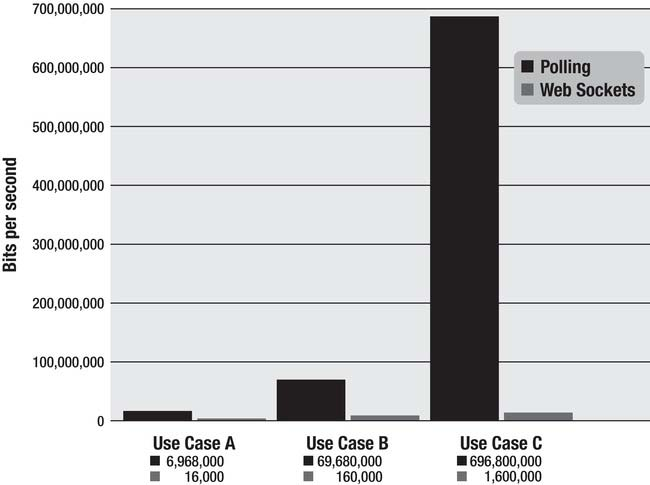
\includegraphics[width=420pt]{img/http-overhead}}\hypertarget{idp5418672}{}%
\label{idp5418672}
}
{{\caption[{Comparison of the unnecessary network overhead between the HTTP polling and using WebSockets \docbooktolatexcite{pro-html5-programming}{}}]{{{Comparison of the unnecessary network overhead between the HTTP polling and using WebSockets \docbooktolatexcite{pro-html5-programming}{}}}}\label{fig-http-overhead}}}
\end{center}
\end{figure}

Furthermore, in case the server just received the data and sent the response to the client, there is a {``}blind window{''} when the server cannot notify the client. Whole push system is blocked until the response is received by the client, processed and new request is delivered back to the server. Considering also the possible packet loss and required retransmission in TCP protocol, the delay can be even longer than double bandwidth latency. \docbooktolatexcite{rfc-bidirectional-http}{}
\subsection{HTTP streaming\index{HTTP!streaming}}
\label{chap-http-streaming}\hypertarget{chap-http-streaming}{}%

HTTP streaming is slightly different method than long polling, although they are confused one with the other very often. What is mutual for both of the approaches is the client initializing the communication with HTTP request. The server also sends the update as the part of the HTTP response. The main difference is that once the server initializes the response and sends the data, it does not terminate the response and keeps the HTTP connection opened. Meanwhile, the client listens to the response stream and reads the data pushed from the server. When any new data springs up on the server side, it is concatenated to the one existing response stream. \docbooktolatexcite{rfc-bidirectional-http}{} See the schema on TODO figure.

It is very important not to confuse HTTP streaming with the {``}persistent{''} HTTP requests. As said at the beginning of this chapter, declaring {\texttt{{Connection: Keep-Alive}}} does not allow the server to issue multiple responses to a single request. Such behaviour would be serious violation of HTTP protocol. Instead, the server can declare {\texttt{{Transfer-Encoding: chunked}}}\index{HTTP!chunked response} status in the response header and send the response split into separate pieces, as show below (chunk of zero length stands for the end of the response): \docbooktolatexcite{rfc-bidirectional-http}{}

\begin{Verbatim}[fontsize=\small]
HTTP/1.1 200 OK
Content-Type: text/plain
Transfer-Encoding: chunked

25
This is the data in the first chunk

1C
and this is the second one

0
\end{Verbatim}

The main drawback of HTTP streaming can be generally called buffering. There is no requirement for both the client and any intermediary (proxies, gateways, etc.) to handle the incoming data until whole response is sent. Therefore, all parts of the response could be kept by the proxy and the messages (single HTTP response chunks) are not delivered to the client until whole response is sent. Similarly, when the response consists of JavaScript statements, the browser does not have to execute them before whole response is obtained (yet, most of the browsers execute it immediately). In such cases, HTTP streaming will not work. \docbooktolatexcite{rfc-bidirectional-http}{}

% ------------------------   
% Section 
\section{WebSockets}
\label{chap-ws}\hypertarget{chap-ws}{}%

Although the World Wide Web with HTTP request/response schema has never been intended to server as RTC platform, the contemporary applications require such functionality and the developers started to bend the protocol in the undesirable way. Most of the patterns described in \hyperlink{chap-http-streaming}{Section�{\ref{chap-http-streaming}}} do their jobs and one can achieve sufficient two-way communication, but there are certain performance issues and drawbacks which make them difficult to use. At least, those techniques carry HTTP header overhead which is unnecessary for standard bidirectional streams. Therefore, brand new standard for creating full-duplex communication channels between the web browser and the server has been created. The technology is called {\em{WebSockets}}\index{WebSocket} (sometimes shortened as WS) and it stands for a communication protocol layered over TCP along with the browser API for web developers. Anyway, not even WebSockets are allowed to access wider network, the connection possibilities are limited only to the dedicated WS servers (usually HTTP servers with additional module for WS support attached). \docbooktolatexcite{js-definitive-guide}{}

Similarly as in HTTP, there is an unencrypted version of WebSockets working directly on top of TCP connection. The simpliest way to recognize such connection is WebSocket URI\index{WebSocket!URI} beginning with {\texttt{{ws://}}}. It should not be used on account of two reasons. The first one, quite obvious, is security - the communication can be captured during the transmission. Transparent proxy servers are the second reason. If an unencrypted WebSocket connection is used, the browser is unaware of the transparent proxy and as a result, the WebSocket connection is most likely to fail. \docbooktolatexcite{ws-proxy}{}\docbooktolatexcite{definitive-guide-to-ws}{} As opposite, there is a secure way how to use WebSockets. WebSockets Secure (WSS)\index{WebSocket!Secure} protocol is standard WS wrapped in TLS tunnel, similarly as HTTP can be transmitted over TLS layer. When using WSS, the URI begins with {\texttt{{wss://}}} and it uses port 443 by default. \docbooktolatexcite{definitive-guide-to-ws}{}
\subsection{Handshake}
\label{idp5451424}\hypertarget{idp5451424}{}%

Alike any other multilateral protocol WebSockets need to perform a handshake before actual transmission can take place. During the handshake, the connection is established and both peers acknowledge the properties of the communication.

Since WebSockets emerged as HTTP supplement, the handshake is initialized by HTTP request\label{idp5453088}\begingroup\catcode`\#=12\footnote{
According to RFC6455, the protocol is designed to work over HTTP ports 80 and 443 as well to support HTTP proxies. However, the design is not limited to HTTP and the future implementations can use simplier handshake over a dedicated port. \docbooktolatexcite{rfc-ws}{}
}\endgroup\docbooktolatexmakefootnoteref{idp5453088} initialized by the client. The client sends the request as follows: \docbooktolatexcite{rfc-ws}{}

\begin{Verbatim}[fontsize=\small]
GET /chat HTTP/1.1
Host: server.example.com
Upgrade: websocket
Connection: Upgrade
Sec-WebSocket-Key: dGhlIHNhbXBsZSBub25jZQ==
Origin: http://example.com
Sec-WebSocket-Protocol: chat, superchat
Sec-WebSocket-Version: 13
\end{Verbatim}

Let us have a look what each of the lines means. The first two lines are obvious, they represent typical HTTP GET request. Specifying {\texttt{{Host}}} is important for the server to be able to handle multiple virtual hosts on single IP address. The following two lines, {\texttt{{Upgrade: websocket}}} and {\texttt{{Connection: Upgrade}}}, are the most important. The client informs the server about the desire to use WS. The rest of the request stands for additional information for the server to be able to respond correctly - RFC 6455 describes them in detail.

The server should send HTTP response looking similar as this example: \docbooktolatexcite{rfc-ws}{}

\begin{Verbatim}[fontsize=\small]
HTTP/1.1 101 Switching Protocols
Upgrade: websocket
Connection: Upgrade
Sec-WebSocket-Accept: s3pPLMBiTxaQ9kYGzzhZRbK+xOo=
\end{Verbatim}

Number 101 on the first line of the response stands for HTTP status code {\texttt{{Switching Protocols}}}, \docbooktolatexcite{rfc-http}{} which means the server supports WebSockets and the connection can be established. Any status code other than 101 indicates that the WebSocket handshake has not completed and that the semantics of HTTP still apply. \docbooktolatexcite{rfc-ws}{}

{\texttt{{Sec-WebSocket-Key}}} is random secret issued by the client and added to the initial protocol-switching request. The server is supposed to concatenate the secret with Globally Unique Identifier (GUID) "258EAFA5-E914-47DA- 95CA-C5AB0DC85B11" and hash the result with SHA-1 algorithm. The resultis returned as {\texttt{{Sec-WebSocket-Accept}}} header field, base64-encoded. \docbooktolatexcite{rfc-ws}{} However, there seems to be a security issue here. If the initial request is not sent over encrypted HTTP connection (HTTPS), it can be caught by a third party. Since the server does not authenticate in any way and the algorithm does not contain any server secret, the third party attacker could fake the response and pretend to be the server.
\subsection{Frames and masking}
\label{idp5464784}\hypertarget{idp5464784}{}%

All the data sent via WebSockets protocol is chunked into frames, working similarly as TCP frames. All the transmission features are handled by the WebSocket API and the transmission is transparent for the application layer above (for example JavaScript API) so that that every message appears in the same state as it was sent.

There are several special features concerning WS frames, one of the interesting is masking\index{masking}. The payload data of every frame sent from the client is XORed by the masking key of 32-bit size. The purpose of masking is to prevent any third party from picking any part of the payload and reading it. The other goal might be distinguishing the server stream from the client stream instantly since client-to-server frames always must be masked and server-to-client frames must not be masked under any circumstances. In addition, WS peers have to use masking even if the communication is running on top of TLS layer so the {``}encryption{''} function is pointless. \docbooktolatexcite{rfc-ws}{} The security function of masking is also questionable because the masking key is included in the frame header. The only reason is preventing from random cross-protocol attacks. \docbooktolatexcite{pro-html5-programming}{}
\subsection{JavaScript API}
\label{idp5469680}\hypertarget{idp5469680}{}%

% ------------------------   
% Section 
\section{Existing RTC frameworks}
\label{idp5470832}\hypertarget{idp5470832}{}%

Actually, there are other options such as using various browser plugins (e.g. Adobe Flash) to provide the base layer for TCP connections, but such tools has not been used within this thesis and are not further dealt with.

Describe other approaches to RTC in WB than XMPP. Tell why we didn't use them (or that we used - OpenTok).

Mention:

Bayeux: http://svn.cometd.org/trunk/bayeux/bayeux.html

OpenTok

SignalR (.NET)

WebRTC (http://www.webrtc.org/)

Google hangouts API

% -------------------------------------------------------------
% Chapter Extensible Messaging and Presence Protocol 
% ------------------------------------------------------------- 	
\chapter{Extensible Messaging and Presence Protocol}
\label{chap-xmpp}\hypertarget{chap-xmpp}{}%

Extensible Messaging and Presence Protocol (XMPP) technologies were invented by Jeremie Miller in 1998. \docbooktolatexcite{xmpp-the-definitive-guide}{} It is one of the most widespread technologies for instant messaging (IM),\label{idp5476928}\begingroup\catcode`\#=12\footnote{
Acutally, the IM client or even the techology itself is sometimes called {``}Instant Messenger{''}. This term is registered as a trademark by AOL company. \docbooktolatexcite{aol-trademarks}{}
}\endgroup\docbooktolatexmakefootnoteref{idp5476928} i.e. exchanging the text or multimedia data between several endpoints. The {``}native{''} implementation of XMPP works right on top of TCP protocol: XMPP endpoint (called client as it represents the first actor in client-server architecture) opens long-lived TCP connection. Then, both the client and the server negotiate and open XML streams so there is one stream in each direction. \docbooktolatexcite{xmpp-the-definitive-guide}{} When the connection is established, both client and server can push any changes as XML elements to the stream and the other side obtains them immediately. Usual XMPP clients are standalone applications able to open TCP connection and listen to the stream opened by the server.

% ------------------------   
% Section 
\section{Fundamental bulding blocks in XMPP}
\label{idp5480160}\hypertarget{idp5480160}{}%

Mention the terms as stanza, roster, describe the subscription mechanism.

% ------------------------   
% Section 
\section{XMPP over BOSH}
\label{chap-bosh}\hypertarget{chap-bosh}{}%

Describe BOSH (http://xmpp.org/extensions/xep-0124.html)

and XMPP Over BOSH (http://xmpp.org/extensions/xep-0206.html).

Later on, description of BOSH extension, including the advantages and limitations. Describe also the connection to HTTP protocol.

% ------------------------   
% Section 
\section{XMPP over WebSockets}
\label{chap-xmpp-ws}\hypertarget{chap-xmpp-ws}{}%

Usually if the WebSockets are used, the XMPP server needs one extra layer, usually implemented as the server plugin, to be able to communicate directly with the web browser.

http://blog.superfeedr.com/xmpp-over-websockets/

luajit - lua jit compiler

It was neccessary to install: apt bal�ky luajit + liblua5.1-bitop0

TODO create diagram here (XMPP server - plugin - incoming connection vs xmpp server - standard connection).

% ------------------------   
% Section 
\section{Jingle}
\label{idp5487136}\hypertarget{idp5487136}{}%

Jingle extension - multimedia.

http://xmpp.org/extensions/xep-0166.html

% ------------------------   
% Section 
\section{Inter-process communication}
\label{idp5488672}\hypertarget{idp5488672}{}%

Pub-sub extensions for inter-process communication.

http://xmpp.org/extensions/xep-0060.html

% -------------------------------------------------------------
% Chapter XMPP client in JavaScript 
% ------------------------------------------------------------- 	
\chapter{XMPP client in JavaScript}
\label{chap-xmpp-in-javascript}\hypertarget{chap-xmpp-in-javascript}{}%

Describe the tools that can be used to implement RTC in WB (and which were used to implement Celebrio Talker)

Strophe (simple XMPP in Javascript)

Strophe connecting/attaching - security issues. TODO programming

Strophe plugins

Possible server-side implementations (JAXL, XMPPHP, ...)

% -------------------------------------------------------------
% Chapter Talker 
% ------------------------------------------------------------- 	
\chapter{Talker}
\label{chap-talker}\hypertarget{chap-talker}{}%

Describe the Talker application in Celebrio.

Mention what we expected from the app (value proposition)

Then, application analysis, design and implmementation.

Describe the architecture and used tools\&frameworks: JS + Ember.js, OpenTok, WebSockets in new OpenTok

Don't forget to use UML: use case diagram, class diagram (if any), sequence/action diagram

% ------------------------   
% Section 
\section{Ember.js}
\label{idp5496624}\hypertarget{idp5496624}{}%

Describe Javascript client-side MVC frameworks overall, compare, tell why we used Ember
\subsection{Subsection about Ember...}
\label{idp5497760}\hypertarget{idp5497760}{}%

% -------------------------------------------------------------
% Chapter Inter-process Communication Framework 
% ------------------------------------------------------------- 	
\chapter{Inter-process Communication Framework}
\label{chap-inter-process}\hypertarget{chap-inter-process}{}%

Implement and describe framework for inter-process communication in Celebrio.

First, the lightweight one (which we already have), then implement the "heavy" one, if there's enough time.

% -------------------------------------------------------------
% Chapter Conclusion 
% ------------------------------------------------------------- 	
\chapter{Conclusion}
\label{idp5501040}\hypertarget{idp5501040}{}%

conclusion

% ------------------------   
% Section 
\section{Another part of the conclusion}
\label{idp5502064}\hypertarget{idp5502064}{}%

Another part of the conclusion... just to have subchapter here
% ------------------------------------------- 
%
%  Bibliography - chapter
%
% ------------------------------------------- 
\begin{thebibliography}{123}\hypertarget{idp5503344}{}

% ............. biblioentry 
\bibitem{aol-trademarks}\docbooktolatexbibaux{idp5571776}{aol-trademarks}
\hypertarget{idp5571776}
AOL Inc.: \emph{AOL Trademark List}, 3/15/2011 [retrieved 2/20/2013], from {\textless}\url{http://legal.aol.com/trademarks/}{\textgreater}. 

% ............. biblioentry 
\bibitem{apache-core-features}\docbooktolatexbibaux{idp5611952}{apache-core-features}
\hypertarget{idp5611952}
The Apache Software Foundation: \emph{Apache Core Features}, 2013 [retrieved 2/23/2013], from {\textless}\url{http://httpd.apache.org/docs/2.2/mod/core.html}{\textgreater}. 

% ............. biblioentry 
\bibitem{async-javascript}\docbooktolatexbibaux{idp5527584}{async-javascript}
\hypertarget{idp5527584}
Burnham, T.: \emph{Async JavaScript}, The Pragmatic Programmers, 2012, 978-1-93778-527-7, 104. 

% ............. biblioentry 
\bibitem{brian-stats-tweet}\docbooktolatexbibaux{idp5586048}{brian-stats-tweet}
\hypertarget{idp5586048}
Staatss, B. (Brianstaats): \emph{{``}If you have to customize 1/5 of a reusable component, its likely better to write it from scratch @trek at \#embercamp{''}}, 2/15/2013 [retrieved 2/23/2013], Tweet. 

% ............. biblioentry 
\bibitem{celebrio-system}\docbooktolatexbibaux{idp5558112}{celebrio-system}
\hypertarget{idp5558112}
Donko, P. and Kunc, P. and Nov�k, M. and Smolka, P. and Volmut, J.: \emph{Celebrio System}, 2013 [retrieved 2/19/2013], from {\textless}\url{http://www.celebriosoftware.com/celebrio-system}{\textgreater}. 

% ............. biblioentry 
\bibitem{definitive-guide-to-html5}\docbooktolatexbibaux{idp5518272}{definitive-guide-to-html5}
\hypertarget{idp5518272}
Freeman, A.: \emph{The Definitive Guide to HTML5 - TODO cite from page 873
      multimedia chapter}, Apress, 2011, 978-1-4302-3960-4, 1080. 

% ............. biblioentry 
\bibitem{definitive-guide-to-ws}\docbooktolatexbibaux{idp5510976}{definitive-guide-to-ws}
\hypertarget{idp5510976}
Wang, V. and Salim, F. and Moskovits, P.: \emph{The Definitive Guide to HTML5 WebSocket}, Apress, 2012, 978-1430247401, 210 (140, 156, ). 

% ............. biblioentry 
\bibitem{elderly-questionnaires}\docbooktolatexbibaux{idp5566672}{elderly-questionnaires}
\hypertarget{idp5566672}
Smolka, P. and Nov�k, M.: \emph{Elderly people and the computers}, 2/11/2013 [retrieved 2/19/2013], from {\textless}\url{http://infogr.am/Seniori-a-pocitace}{\textgreater}. 

% ............. biblioentry 
\bibitem{facebook-usage}\docbooktolatexbibaux{idp5549664}{facebook-usage}
\hypertarget{idp5549664}
Olanoff, D.: \emph{Facebook Announces Monthly Active Users Were At 1.01 Billion As
      Of September 30th}, TechCrunch, 10/23/2012 [retrieved 2/19/2013], from {\textless}\url{http://techcrunch.com/2012/10/23/facebook-announces-monthly-active-users-were-at-1-01-billion-as-of-september-30th/}{\textgreater}. 

% ............. biblioentry 
\bibitem{fb-chat}\docbooktolatexbibaux{idp5582480}{fb-chat}
\hypertarget{idp5582480}
Facebook Developers: \emph{Facebook Chat API}, 2/12/2013 [retrieved 2/20/2013], from http://xmpp.org/about-xmpp/history/ {\textless}\url{http://legal.aol.com/trademarks/}{\textgreater}. 

% ............. biblioentry 
\bibitem{fb-erlang}\docbooktolatexbibaux{idp5589392}{fb-erlang}
\hypertarget{idp5589392}
Letuchy, E.: \emph{Facebook Chat}, 5/14/2008 [retrieved 2/23/2013], from {\textless}\url{https://www.facebook.com/note.php?note_id=14218138919}{\textgreater}. 

% ............. biblioentry 
\bibitem{gtalk}\docbooktolatexbibaux{idp5578912}{gtalk}
\hypertarget{idp5578912}
Google Developers: \emph{Google Talk Developer Documentation}, 3/23/2012 [retrieved 2/20/2013], from {\textless}\url{https://developers.google.com/talk/talk_developers_home}{\textgreater}. 

% ............. biblioentry 
\bibitem{internet-usage}\docbooktolatexbibaux{idp5545712}{internet-usage}
\hypertarget{idp5545712}
Miniwatts Marketing Group: \emph{Internet Users in the World - 2012 Q2}, Internet World Stats, 2/17/2013 [retrieved 2/19/2013], from {\textless}\url{http://www.internetworldstats.com/stats.htm}{\textgreater}. 

% ............. biblioentry 
\bibitem{js-definitive-guide}\docbooktolatexbibaux{idp5522976}{js-definitive-guide}
\hypertarget{idp5522976}
Flanagan, D.: \emph{JavaScript: The Definitive Guide}, O'Reilly Media, 2011, 978-0-596-80552-4, 1100 (333). 

% ............. biblioentry 
\bibitem{pro-html5-programming}\docbooktolatexbibaux{idp5538800}{pro-html5-programming}
\hypertarget{idp5538800}
Lubbers, P. and Salim, F. and Albers, B.: \emph{Pro HTML5 Programming}, Apress, 2011, 978-1-4302-3864-5, 352 (165, ...). 

% ............. biblioentry 
\bibitem{realtime-web-apps}\docbooktolatexbibaux{idp5532576}{realtime-web-apps}
\hypertarget{idp5532576}
Lengstorf, J. and Leggetter, P.: \emph{Realtime Web Apps}, Apress, 2013, 978-1430246206, 400. 

% ............. biblioentry 
\bibitem{rfc-bidirectional-http}\docbooktolatexbibaux{idp5615136}{rfc-bidirectional-http}
\hypertarget{idp5615136}
Loreto, S. and Saint-Andre, P. and Salsano, S. and Wilkins, G.: \emph{Known Issues and Best Practices for the Use of Long Polling and
      Streaming in Bidirectional HTTP}, 4/2011 [retrieved 2/23/2013], from {\textless}\url{http://www.ietf.org/rfc/rfc6202.txt}{\textgreater}. 

% ............. biblioentry 
\bibitem{rfc-http}\docbooktolatexbibaux{idp5600320}{rfc-http}
\hypertarget{idp5600320}
Fielding, R. and Gettis, J. and Mogul, J. and Frystyk, H. and Masinter, L. and Leach, P. and Berners-Lee, T.: \emph{Hypertext Transfer Protocol -- HTTP/1.1}, 6/1999 [retrieved 2/23/2013], from {\textless}\url{http://www.w3.org/Protocols/rfc2616/rfc2616.html}{\textgreater}. 

% ............. biblioentry 
\bibitem{rfc-ws}\docbooktolatexbibaux{idp5623040}{rfc-ws}
\hypertarget{idp5623040}
Fette, I. and Melnikov, A.: \emph{The WebSocket Protocol}, 12/2011 [retrieved 2/24/2013], Internet Engineering Task Force (IETF), from {\textless}\url{http://tools.ietf.org/html/rfc6455}{\textgreater}. 

% ............. biblioentry 
\bibitem{ria}\docbooktolatexbibaux{idp5554352}{ria}
\hypertarget{idp5554352}
Ward, J.: \emph{What is a Rich Internet Application?}, 10/17/2007 [retrieved 2/19/2013], from {\textless}\url{http://www.jamesward.com/2007/10/17/what-is-a-rich-internet-application/}{\textgreater}. 

% ............. biblioentry 
\bibitem{skype-license}\docbooktolatexbibaux{idp5592960}{skype-license}
\hypertarget{idp5592960}
Smith, A.: \emph{Does SkypeKit work on Android?}, 8/7/2012 [retrieved 2/23/2013], from {\textless}\url{http://devforum.skype.com/t5/SkypeKit-FAQs/Does-SkypeKit-work-on-Android/m-p/16490/thread-id/78}{\textgreater}. 

% ............. biblioentry 
\bibitem{skype-uri}\docbooktolatexbibaux{idp5597136}{skype-uri}
\hypertarget{idp5597136}
Microsoft: \emph{Skype URIs}, 2013 [retrieved 2/23/2013], from {\textless}\url{http://dev.skype.com/skype-uri}{\textgreater}. 

% ............. biblioentry 
\bibitem{ws-proxy}\docbooktolatexbibaux{idp5629680}{ws-proxy}
\hypertarget{idp5629680}
Lubbers, P.: \emph{How HTML5 Web Sockets Interact With Proxy Servers}, 3/16/2011 [retrieved 2/24/2013], InfoQ, from {\textless}\url{http://tools.ietf.org/html/rfc6455}{\textgreater}. 

% ............. biblioentry 
\bibitem{xmpp-history}\docbooktolatexbibaux{idp5575344}{xmpp-history}
\hypertarget{idp5575344}
The XMPP Standards Foundation: \emph{History of XMPP}, 1/27/2010 [retrieved 2/20/2013], from http://xmpp.org/about-xmpp/history/ {\textless}\url{http://legal.aol.com/trademarks/}{\textgreater}. 

% ............. biblioentry 
\bibitem{xmpp-the-definitive-guide}\docbooktolatexbibaux{idp5503600}{xmpp-the-definitive-guide}
\hypertarget{idp5503600}
Saint-Andre, P. and Smith, K. and Tron�on, R.: \emph{XMPP: The Definitive Guide}, Sebastopol: O'Reilly, 2009, 978-0-596-52126-4, 310 (7, 16, ). 

\end{thebibliography}
\addcontentsline{toc}{chapter}{Bibliography}
\setlength\saveparskip\parskip
\setlength\saveparindent\parindent
\begin{dbtolatexindex}{idp5634912}{}
\setlength\tempparskip\parskip \setlength\tempparindent\parindent
\parskip\saveparskip \parindent\saveparindent
\noindent \indexspace
\parskip\tempparskip
\parindent\tempparindent
\makeatletter\@input@{\jobname.ind}\makeatother
\addcontentsline{toc}{chapter}{Index}
\end{dbtolatexindex}

\newcommand{\dbappendix}[1]{\chapter{#1}}%
% ------------------------------------------------------------- 
% Appendices start here
% -------------------------------------------------------------
\appendix

% -------------------------------------------------------------
% appendix:  Screenshots of the application 
% ------------------------------------------------------------- 	
\dbappendix{Screenshots of the application}
\label{my-appendix}\hypertarget{my-appendix}{}%

Some screenshots from Celebrio Talker

\end{document}

